\documentclass[tikz,border=10pt]{standalone}
\usetikzlibrary{shapes.geometric, arrows.meta, positioning, calc, shadows}

\begin{document}

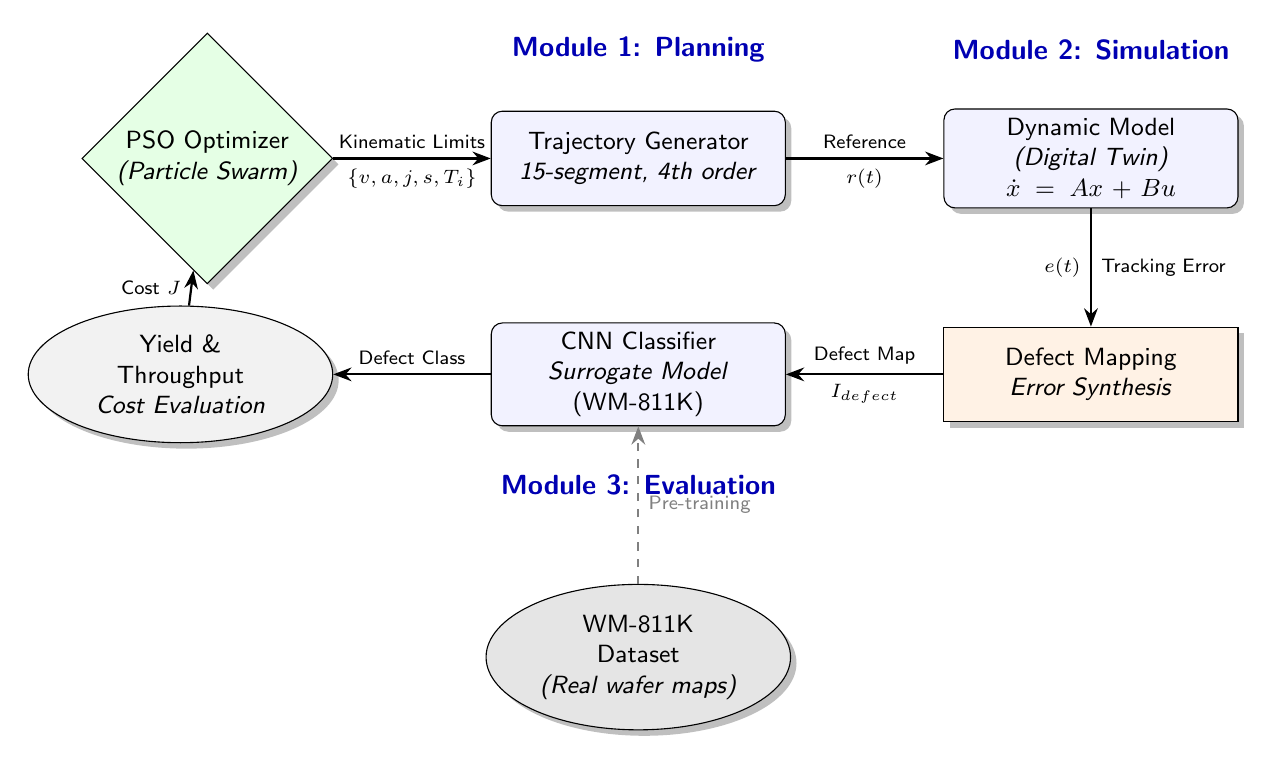
\begin{tikzpicture}[
    node distance=1.5cm and 2cm,
    block/.style={
        rectangle, 
        draw, 
        fill=blue!5, 
        text width=3.5cm, 
        text centered, 
        rounded corners, 
        minimum height=1.2cm,
        font=\sffamily\small,
        drop shadow
    },
    process/.style={
        rectangle, 
        draw, 
        fill=orange!10, 
        text width=3.5cm, 
        text centered, 
        minimum height=1.2cm,
        font=\sffamily\small,
        drop shadow
    },
    optimizer/.style={
        diamond, 
        draw, 
        fill=green!10, 
        text width=2.5cm, 
        text centered, 
        inner sep=0pt,
        font=\sffamily\small,
        drop shadow
    },
    data/.style={
        ellipse, 
        draw, 
        fill=gray!10, 
        text width=2.5cm, 
        text centered, 
        font=\sffamily\small,
        drop shadow
    },
    line/.style={
        draw, 
        -Stealth, 
        thick,
        font=\sffamily\scriptsize
    }
]

    % --- Nodes ---
    
    % Optimizer at the start/loop end
    \node [optimizer] (pso) {PSO Optimizer \\ \textit{(Particle Swarm)}};
    
    % Trajectory Generation
    \node [block, right=of pso] (traj) {Trajectory Generator \\ \textit{15-segment, 4th order}};
    
    % Dynamic Model (Digital Twin)
    \node [block, right=of traj] (model) {Dynamic Model \\ \textit{(Digital Twin)} \\ $\dot{x} = Ax + Bu$};
    
    % Tracking Error & Defect Mapping
    \node [process, below=of model] (defect) {Defect Mapping \\ \textit{Error Synthesis}};
    
    % CNN Surrogate
    \node [block, left=of defect] (cnn) {CNN Classifier \\ \textit{Surrogate Model} \\ (WM-811K)};
    
    % Yield / Cost Function
    \node [data, left=of cnn] (yield) {Yield \& Throughput \\ \textit{Cost Evaluation}};
    
    % External Data Resource
    \node [data, below=2cm of cnn, fill=gray!20] (dataset) {WM-811K Dataset \\ \textit{(Real wafer maps)}};

    % --- Connections ---
    
    % Forward Path
    \draw [line] (pso) -- node[above] {Kinematic Limits} node[below] {$\{v, a, j, s, T_i\}$} (traj);
    \draw [line] (traj) -- node[above] {Reference} node[below] {$r(t)$} (model);
    \draw [line] (model) -- node[right] {Tracking Error} node[left] {$e(t)$} (defect);
    \draw [line] (defect) -- node[above] {Defect Map} node[below] {$I_{defect}$} (cnn);
    \draw [line] (cnn) -- node[above] {Defect Class} (yield);
    
    % Feedback Loop
    \draw [line] (yield) -- node[left] {Cost $J$} (pso);
    
    % Training path for CNN
    \draw [line, dashed, color=gray] (dataset) -- node[right] {Pre-training} (cnn);
    
    % Inputs/Outputs markers
    \node [above=0.5cm of traj, font=\sffamily\bfseries\color{blue!70!black}] {Module 1: Planning};
    \node [above=0.5cm of model, font=\sffamily\bfseries\color{blue!70!black}] {Module 2: Simulation};
    \node [below=0.5cm of cnn, font=\sffamily\bfseries\color{blue!70!black}] {Module 3: Evaluation};

\end{tikzpicture}

\end{document}
